% =============================================================================
%  Planner-Distilled Decision Transformers for Multi-Market BESS Dispatch
%  ArXiv preprint — NeurIPS-style.  SCAFFOLD ONLY.
% -----------------------------------------------------------------------------
%  HOW TO USE (author):
%   - This file is a SKELETON. Every `% TODO(author):` marks text YOU must write.
%   - Numbers marked [FACT] are traced in paper/audit/provenance.tsv — keep them
%     consistent with that table; do not retype from memory.
%   - Figures use \figph{} placeholders until Phase 4 regenerates them from the
%     extended-surface artifacts. Replace with \includegraphics when ready.
%
%  CLAIM MAP
%   C1 (diagnosis/negative) -> Sec. intro + Sec. cloning-ceiling
%   C2 (method/positive)    -> Sec. method + Sec. results
%   C3 (robustness)         -> Sec. market-impact
%  Evidence: report.md §8.2.10 (v1 ladder), §8.2.11 (shipped), paper/audit/*
% =============================================================================
\documentclass{article}

% NeurIPS-style preprint. The package name must match the template's .sty
% (Overleaf "NeurIPS 2026" ships neurips_2026.sty). Also mirror the option the
% template's own \usepackage line uses ([preprint] is standard).
\usepackage[preprint]{neurips_2026}

\usepackage[utf8]{inputenc}
\usepackage[T1]{fontenc}
\usepackage{hyperref}
\usepackage{url}
\usepackage{booktabs}   % \toprule \midrule \bottomrule
\usepackage{amsfonts}
\usepackage{amsmath}
\usepackage{nicefrac}
\usepackage{microtype}
\usepackage{graphicx}
\usepackage{float}   % [H] = pin floats exactly where written
\usepackage{xcolor}

% Placeholder box for figures not yet regenerated (Phase 4).
\newcommand{\figph}[1]{%
  \fbox{\parbox[c][4.5cm][c]{0.86\linewidth}{\centering\small #1}}%
}

\title{Planner-Distilled Decision Transformers Break the\\ Behaviour-Cloning Ceiling in Multi-Market BESS Dispatch}

\author{%
  Hou Nam U (Victor) \\
  \texttt{github.com/mrvictoru/energydecision} \\
}

\begin{document}
\maketitle

% =============================================================================
\begin{abstract}
% TODO(author): 150-200 words. Hit, in order:
%  (1) the problem: offline RL/behaviour cloning has a data ceiling for multi-
%      market (energy + 8 FCAS) battery dispatch;
%  (2) what we do: distil an honest (non-clairvoyant) SDP planning teacher into a
%      standalone Decision Transformer with state-dependent J_t(soc) RTG prompts;
%  (3) headline [FACT]: beats tuned PPO on all four extended identity surfaces
%      (n=30/12/30/6; all paired 95% CIs exclude zero) with no solver at inference,
%      and passes a market-impact gate on 9/9 grid-scale cells.
%  (4) one honest caveat: results are simulator-based (AEMO/NEM data).
\end{abstract}

% =============================================================================
\section{Introduction}
% TODO(author): ~1 page. Structure:
%  - Why BESS dispatch is hard: co-optimise energy + 8 FCAS, degradation matters,
%    online exploration is expensive/risky -> offline learning is attractive.
%  - The catch: offline behaviour cloning is bounded by logged behaviour (C1).
%  - Contribution list (3 bullets = the three claims):
%      C1 diagnose the behaviour-cloning ceiling (and show which levers fail);
%      C2 break it via planner distillation + J_t(soc) prompting;
%      C3 pass a market-impact gate (prompt must be gated by market power).
%  - One-paragraph summary of results with [FACT] numbers.
%  \cite{chen2021decision} \cite{ross2011reduction}

\begin{figure}[htbp]
  \centering
  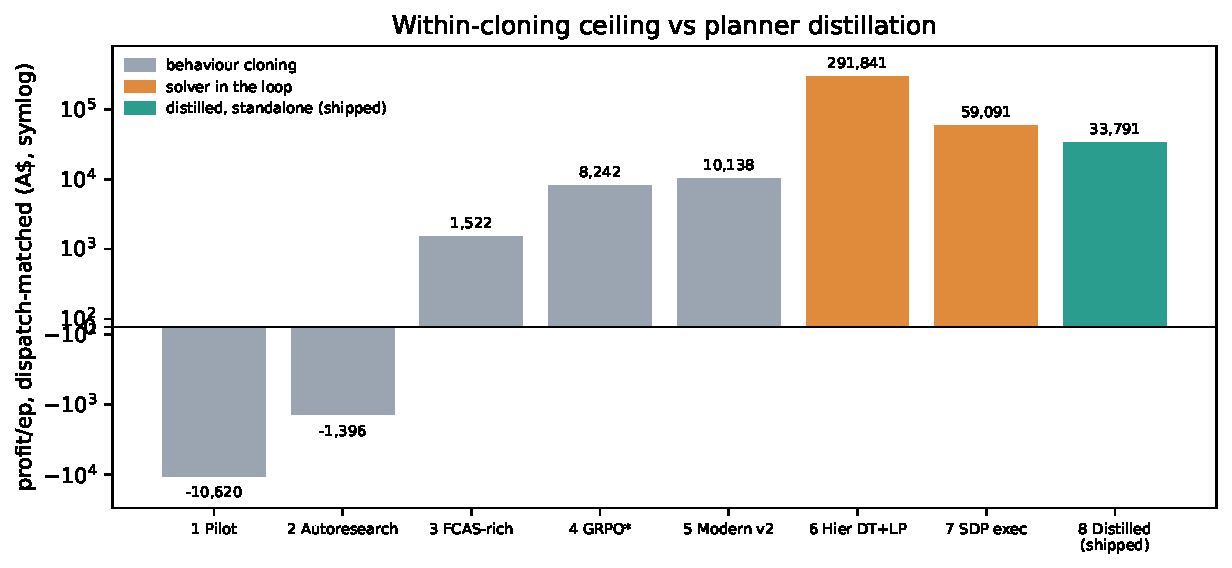
\includegraphics[width=0.9\linewidth]{figures/fig6_ceiling_break.pdf}
  \caption{The behaviour-cloning ceiling and how it is broken. Within the
  cloning paradigm (grey) profit improves then plateaus; solver-in-the-loop
  planners (orange) exceed it but are not deployable; the distilled standalone
  student (teal) keeps the ceiling broken with no solver at inference. Values are
  per-stage evaluation surfaces (report \S8.2.7).}
  \label{fig:ceiling}
\end{figure}

% =============================================================================
\section{Related Work}
% TODO(author): four short paragraphs (see report.md §Related Work / positioning):
%  1. Decision Transformer / offline RL            \cite{chen2021decision,janner2021offline,zheng2022online,li2023qdt}
%  2. Offline-Q alternatives (IQL/CQL)             \cite{kostrikov2022iql,kumar2020cql}
%  3. Planner distillation / imitation              \cite{ross2011reduction}
%  4. BESS scheduling, degradation, benchmarks      \cite{abdulla2016optimal,muenzel2015multifactor,kampker2025modelling,subramanya2022review}

% =============================================================================
\section{Experimental Framework}
\label{sec:setup}
% TODO(author): describe, no results yet:
%  - AEMO/NEM environment: 5-min steps, energy spot + 8 FCAS services,
%    9-dim action (full_fcas).
%  - Degradation model: real-world calendar + cycle aging (Arrhenius), LFP/NMC
%    presets \cite{kampker2025modelling,muenzel2015multifactor}.
%  - Data: historical AEMO dispatch + prices; train on pre-2024, evaluate
%    2024 (identity) and 2025 (OOD). State the no-overlap fact
%    (paper/audit/artifacts/leakage_check.txt).

% =============================================================================
\section{Method}
\label{sec:method}

\subsection{Honest SDP teacher}
% TODO(author): 3 paragraphs.
%  (1) What the teacher sees: cached preprocessed 5-min AEMO data (RRP, demand,
%      8 FCAS prices, gen mix). Forecast = seasonal month x hour mean RRP from
%      pre-2024 only; NO realized future prices enter the loop.
%  (2) The three-stage hierarchy: SOC-waypoint DT (K=8) -> SDP backward induction
%      (degradation-aware per-step wear, deg_calibration) -> greedy current-price
%      FCAS bidder.
%  (3) The free-terminal recursion yields J_t(soc); that becomes the RTG prompt.
%  Pitfall: it is a HYBRID pipeline, not a pure SDP solver.

\subsection{Trajectory corpus}
% TODO(author): random windows (5 regions x short ~14d / medium ~8wk x 4 batteries
%  x 8) -> self-consistent (obs 18-dim, action 9-dim, reward) triples; shipped
%  corpus 320 eps / 3.13M rows; no timestamps stored (leakage caveat).
%  Cite scripts/generate_sdp_dt_trajectories.py.

\subsection{Student Decision Transformer}
% TODO(author): 8x768 GQA, ctx 210, mixed head; loss
%   L = w_a*MSE_a + w_s*MSE_s + w_r*MSE_r
%  with w_a=0.999, w_s=0.002, w_r=0.0001 [FACT, shipped v2cal]. return_scale is
%  auto-calibrated (p90(|J_t|)/scale ~ 10); shipped 23,284.83.
%  Pitfall: quote the SHIPPED weights, not the function defaults.

\subsection{Return-to-go prompting and \texttt{auto} mode}
% TODO(author): RTG = -J_t(soc) looked up per step; auto = j_t_soc on price-taking
%  surfaces, constant rtg0.0 under market impact (robustness, not collapse-avoidance).

\begin{figure}[htbp]
  \centering
  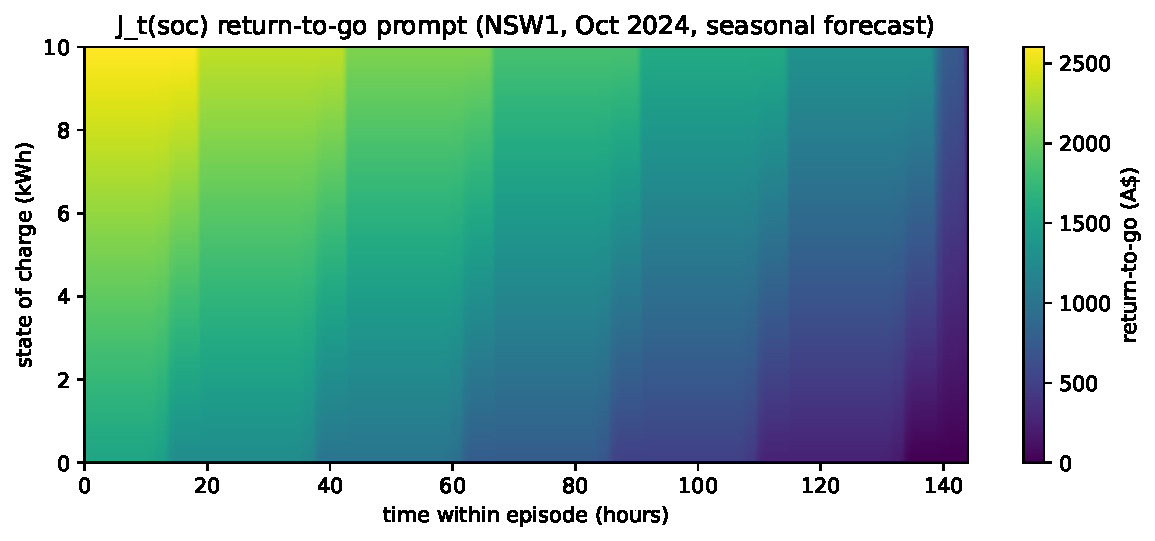
\includegraphics[width=0.92\linewidth]{figures/fig3_jtsoc_heatmap.pdf}
  \caption{The $J_t(\mathrm{soc})$ return-to-go prompt for a representative window
  (NSW1, October 2024, seasonal forecast). Value rises with stored energy and
  decays as the remaining episode shortens; this table supplies the DT's
  state-dependent RTG prompt.}
  \label{fig:jtsoc}
\end{figure}

% =============================================================================
\section{Experiments}
\label{sec:experiments}
% TODO(author):
%  - Surfaces: standard 2024 (5 regions x 6 periods), dispatch-matched (SA1
%    full-year), expanded broad-2024, 2025 OOD. State the cell counts.
%  - Baselines: tuned PPO (Optuna 10 trials, up to 4M steps), fcas_rule,
%    dispatch replay.
%  - Protocol: 5-min steps, one deterministic episode per (scenario, battery)
%    cell; bootstrap 10k over cells + paired Wilcoxon; paired-difference CI is
%    primary. Note PPO run-to-run noise (~1%) as a caveat, and DT determinism.

\subsection{Headline Results}
% [FACT] table — do not retype; mirror paper/audit/artifacts/stagec_v2cal_extended_significance.json
\begin{table}[H]
  \centering
  \caption{Extended identity surfaces (shipped physics-v2 checkpoint,
  \texttt{rtg\_mode="auto"}). \textbf{All four paired-difference 95\% CIs exclude
  zero.} Baselines may show $\sim$1\% run-to-run variation.}
  \label{tab:headline}
  \small
  \begin{tabular}{lrrrrr}
    \toprule
    Surface & $n$ & DT (\$/ep) & PPO (\$/ep) & $\Delta$ (DT$-$PPO) & 95\% CI on $\Delta$ \\
    \midrule
    Standard 2024         & 30 & 16{,}501 & 4{,}303  & $+12{,}198$ & $[9{,}181,\ 14{,}738]$ \\
    Dispatch-matched      & 12 & 33{,}791 & 18{,}818 & $+14{,}973$ & $[4{,}794,\ 22{,}663]$ \\
    Expanded broad-2024   & 30 & 29{,}124 & 4{,}350  & $+24{,}775$ & $[13{,}509,\ 41{,}434]$ \\
    2025 OOD              & 6  & 30{,}791 & 4{,}817  & $+25{,}974$ & $[12{,}708,\ 49{,}850]$ \\
    \bottomrule
  \end{tabular}
\end{table}

\begin{figure}[htbp]
  \centering
  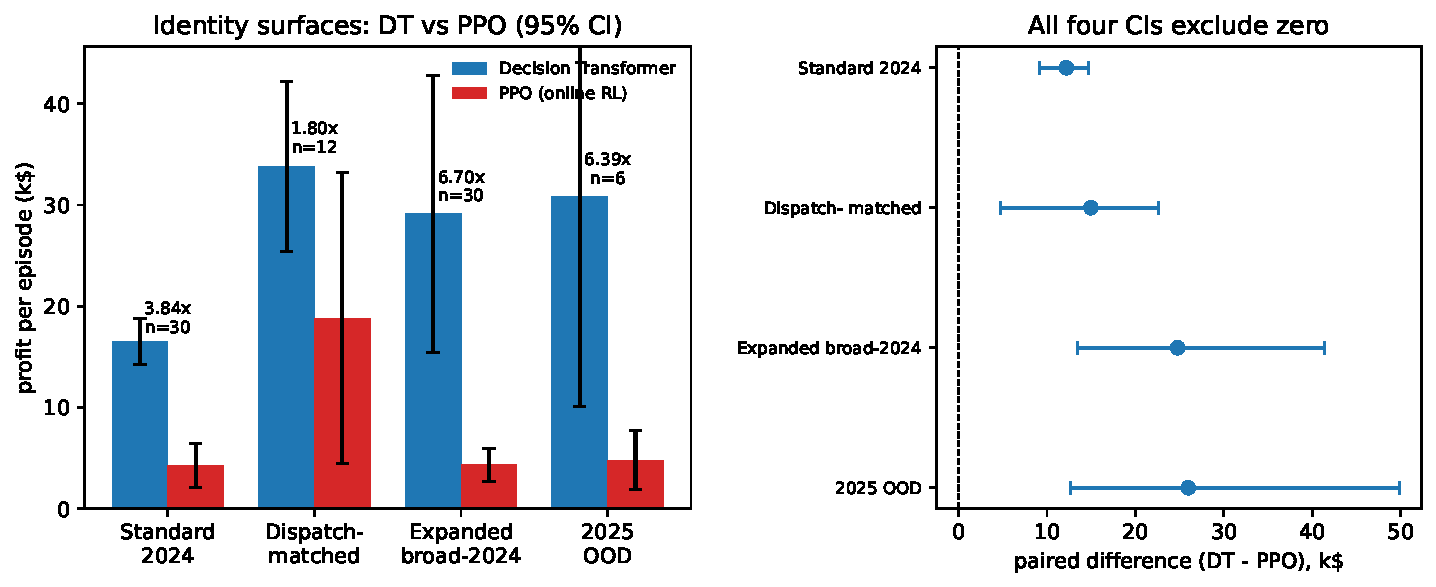
\includegraphics[width=\linewidth]{figures/fig1_main_results.pdf}
  \caption{Decision Transformer vs PPO across the four extended identity
  surfaces. Left: per-episode profit with 95\% bootstrap CIs. Right: the paired
  difference (DT $-$ PPO) with its 95\% CI; all four exclude zero.}
  \label{fig:main}
\end{figure}

\begin{figure}[htbp]
  \centering
  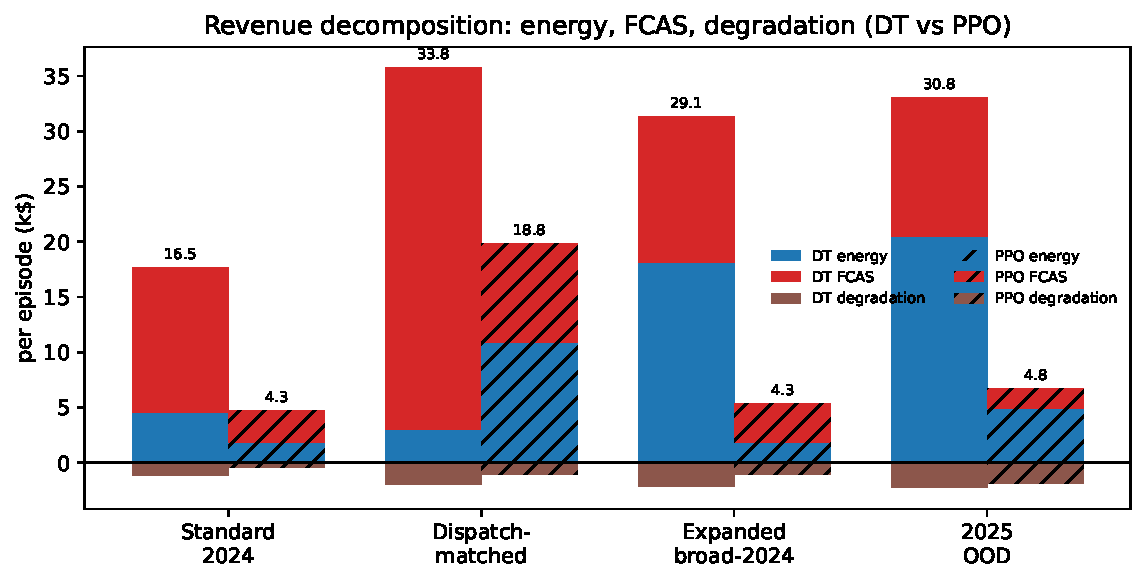
\includegraphics[width=0.85\linewidth]{figures/fig5_revenue_decomposition.pdf}
  \caption{Revenue decomposition (energy, FCAS, degradation) per surface for the
  DT (solid) and PPO (hatched); the annotated number is net profit per episode.
  The DT's advantage is dominated by FCAS capture.}
  \label{fig:revenue}
\end{figure}

% =============================================================================
\section{Market-Impact Gate}
\label{sec:impact}
% TODO(author): C3. Describe the piecewise merit-order impact model, the 9
% grid-scale cells, and the result [FACT]:
%   fixed rtg0.0 fallback beats PPO on 9/9 cells;
%   per-battery ratios small 4.36x / hornsdale 4.71x / torrens 4.67x;
%   paired diff +167,099 USD, 95% CI [101,213, 227,362], p=0.0039.
%   Key point: value-based prompts must be gated by market power (auto mode).

\begin{figure}[htbp]
  \centering
  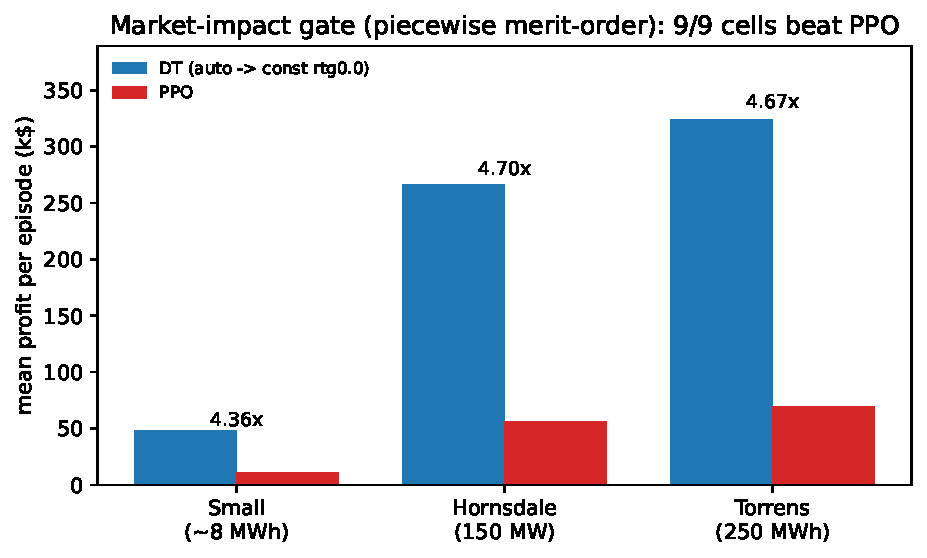
\includegraphics[width=0.8\linewidth]{figures/fig4_impact_resilience.pdf}
  \caption{Market-impact gate (piecewise merit-order). Mean profit per episode
  for the shipped DT (fixed \texttt{rtg0.0} fallback) vs PPO across three
  grid-scale batteries; the DT wins all 9 scenario$\times$battery cells.}
  \label{fig:impact}
\end{figure}

% =============================================================================
\section{Limitations}
\label{sec:limitations}
% TODO(author): be explicit and unprompted:
%  - Simulator-based (sim-to-real is the top open item).
%  - Same-simulator teacher + evaluation: residual circularity (mitigated, not
%    removed, by 2025 OOD + impact gate).
%  - Baseline strength: PPO is tuned (Optuna, 4M steps) but retains noise; the
%    DT is deterministic.
%  - Small n on some surfaces; cells within a region are correlated.
%  - Physics-sensitivity: numbers moved between physics-v1 and v2cal.
%  - Retention: the student keeps 51-91% of the teacher (not >100%).
%  - Stale-cache provenance issue and its fix (paper/audit/artifacts/cache_data_staleness_finding.md).

% =============================================================================
\section{Conclusion}
% TODO(author): 2 short paragraphs — restate C1/C2/C3 and the one-line takeaway:
% "most of the planner, none of the solver", plus the sim-to-real next step.

% =============================================================================
\begin{ack}
% TODO(author): optional. If you used AI assistance, disclose it here per the
% venue policy (code assistance is normal; all analysis/claims are the author's).
\end{ack}

\bibliographystyle{plainnat}
\bibliography{references}

% =============================================================================
\appendix
\section{Provenance and Reproducibility}
% TODO(author): point to:
%  - paper/audit/provenance.tsv (every headline number -> artifact + command)
%  - paper/environment.txt (frozen environment), tag preprint-v1
%  - HF artifacts: model mrvictoru/energydecision-dt-v2-sdp, dataset
%    mrvictoru/AEMO_simulated_trade_sdp
%  - leakage check, determinism probe, cache-key fix
%  - test suite: 387 passing

\end{document}
